% This is the Reed College LaTeX thesis template. Most of the work
% for the document class was done by Sam Noble (SN), as well as this
% template. Later comments etc. by Ben Salzberg (BTS). Additional
% restructuring and APA support by Jess Youngberg (JY).
% Your comments and suggestions are more than welcome; please email
% them to cus@reed.edu
%
% See http://web.reed.edu/cis/help/latex.html for help. There are a
% great bunch of help pages there, with notes on
% getting started, bibtex, etc. Go there and read it if you're not
% already familiar with LaTeX.
%
% Any line that starts with a percent symbol is a comment.
% They won't show up in the document, and are useful for notes
% to yourself and explaining commands.
% Commenting also removes a line from the document;
% very handy for troubleshooting problems. -BTS

% As far as I know, this follows the requirements laid out in
% the 2002-2003 Senior Handbook. Ask a librarian to check the
% document before binding. -SN

%%
%% Preamble
%%
% \documentclass{<something>} must begin each LaTeX document
\documentclass[12pt,twoside]{reedthesis}
% Packages are extensions to the basic LaTeX functions. Whatever you
% want to typeset, there is probably a package out there for it.
% Chemistry (chemtex), screenplays, you name it.
% Check out CTAN to see: http://www.ctan.org/
%%
\usepackage{graphicx,latexsym}
\usepackage{amsmath}
\usepackage{amssymb,amsthm}
\usepackage{longtable,booktabs,setspace}
\usepackage{chemarr} %% Useful for one reaction arrow, useless if you're not a chem major
\usepackage[hyphens]{url}
% Added by CII
\usepackage{hyperref}
\usepackage{lmodern}
\usepackage{float}
\floatplacement{figure}{H}
% End of CII addition
\usepackage{rotating}

% Next line commented out by CII
%%% \usepackage{natbib}
% Comment out the natbib line above and uncomment the following two lines to use the new
% biblatex-chicago style, for Chicago A. Also make some changes at the end where the
% bibliography is included.
%\usepackage{biblatex-chicago}
%\bibliography{thesis}


% Added by CII (Thanks, Hadley!)
% Use ref for internal links
\renewcommand{\hyperref}[2][???]{\autoref{#1}}
\def\chapterautorefname{Chapter}
\def\sectionautorefname{Section}
\def\subsectionautorefname{Subsection}
% End of CII addition

% Added by CII
\usepackage{caption}
\captionsetup{width=5in}
% End of CII addition

% \usepackage{times} % other fonts are available like times, bookman, charter, palatino

% Syntax highlighting #22
  \usepackage{color}
  \usepackage{fancyvrb}
  \newcommand{\VerbBar}{|}
  \newcommand{\VERB}{\Verb[commandchars=\\\{\}]}
  \DefineVerbatimEnvironment{Highlighting}{Verbatim}{commandchars=\\\{\}}
  % Add ',fontsize=\small' for more characters per line
  \usepackage{framed}
  \definecolor{shadecolor}{RGB}{248,248,248}
  \newenvironment{Shaded}{\begin{snugshade}}{\end{snugshade}}
  \newcommand{\KeywordTok}[1]{\textcolor[rgb]{0.13,0.29,0.53}{\textbf{{#1}}}}
  \newcommand{\DataTypeTok}[1]{\textcolor[rgb]{0.13,0.29,0.53}{{#1}}}
  \newcommand{\DecValTok}[1]{\textcolor[rgb]{0.00,0.00,0.81}{{#1}}}
  \newcommand{\BaseNTok}[1]{\textcolor[rgb]{0.00,0.00,0.81}{{#1}}}
  \newcommand{\FloatTok}[1]{\textcolor[rgb]{0.00,0.00,0.81}{{#1}}}
  \newcommand{\ConstantTok}[1]{\textcolor[rgb]{0.00,0.00,0.00}{{#1}}}
  \newcommand{\CharTok}[1]{\textcolor[rgb]{0.31,0.60,0.02}{{#1}}}
  \newcommand{\SpecialCharTok}[1]{\textcolor[rgb]{0.00,0.00,0.00}{{#1}}}
  \newcommand{\StringTok}[1]{\textcolor[rgb]{0.31,0.60,0.02}{{#1}}}
  \newcommand{\VerbatimStringTok}[1]{\textcolor[rgb]{0.31,0.60,0.02}{{#1}}}
  \newcommand{\SpecialStringTok}[1]{\textcolor[rgb]{0.31,0.60,0.02}{{#1}}}
  \newcommand{\ImportTok}[1]{{#1}}
  \newcommand{\CommentTok}[1]{\textcolor[rgb]{0.56,0.35,0.01}{\textit{{#1}}}}
  \newcommand{\DocumentationTok}[1]{\textcolor[rgb]{0.56,0.35,0.01}{\textbf{\textit{{#1}}}}}
  \newcommand{\AnnotationTok}[1]{\textcolor[rgb]{0.56,0.35,0.01}{\textbf{\textit{{#1}}}}}
  \newcommand{\CommentVarTok}[1]{\textcolor[rgb]{0.56,0.35,0.01}{\textbf{\textit{{#1}}}}}
  \newcommand{\OtherTok}[1]{\textcolor[rgb]{0.56,0.35,0.01}{{#1}}}
  \newcommand{\FunctionTok}[1]{\textcolor[rgb]{0.00,0.00,0.00}{{#1}}}
  \newcommand{\VariableTok}[1]{\textcolor[rgb]{0.00,0.00,0.00}{{#1}}}
  \newcommand{\ControlFlowTok}[1]{\textcolor[rgb]{0.13,0.29,0.53}{\textbf{{#1}}}}
  \newcommand{\OperatorTok}[1]{\textcolor[rgb]{0.81,0.36,0.00}{\textbf{{#1}}}}
  \newcommand{\BuiltInTok}[1]{{#1}}
  \newcommand{\ExtensionTok}[1]{{#1}}
  \newcommand{\PreprocessorTok}[1]{\textcolor[rgb]{0.56,0.35,0.01}{\textit{{#1}}}}
  \newcommand{\AttributeTok}[1]{\textcolor[rgb]{0.77,0.63,0.00}{{#1}}}
  \newcommand{\RegionMarkerTok}[1]{{#1}}
  \newcommand{\InformationTok}[1]{\textcolor[rgb]{0.56,0.35,0.01}{\textbf{\textit{{#1}}}}}
  \newcommand{\WarningTok}[1]{\textcolor[rgb]{0.56,0.35,0.01}{\textbf{\textit{{#1}}}}}
  \newcommand{\AlertTok}[1]{\textcolor[rgb]{0.94,0.16,0.16}{{#1}}}
  \newcommand{\ErrorTok}[1]{\textcolor[rgb]{0.64,0.00,0.00}{\textbf{{#1}}}}
  \newcommand{\NormalTok}[1]{{#1}}

% To pass between YAML and LaTeX the dollar signs are added by CII
\title{Forecasting Constituents of the MSCI Minimum Volatility Index Through
Logistic Regression}
\author{John A. Gilheany}
% The month and year that you submit your FINAL draft TO THE LIBRARY (May or December)
\date{November 6, 2017}
\division{Statistics}
\advisor{Professor Michael Parzen}
\institution{Harvard College}
\degree{Bachelor of Arts in Statistics (Honors)}
%If you have two advisors for some reason, you can use the following
% Uncommented out by CII
\altadvisor{David Kane}
% End of CII addition

%%% Remember to use the correct department!
\department{Statistics}
% if you're writing a thesis in an interdisciplinary major,
% uncomment the line below and change the text as appropriate.
% check the Senior Handbook if unsure.
%\thedivisionof{The Established Interdisciplinary Committee for}
% if you want the approval page to say "Approved for the Committee",
% uncomment the next line
%\approvedforthe{Committee}

% Added by CII
%%% Copied from knitr
%% maxwidth is the original width if it's less than linewidth
%% otherwise use linewidth (to make sure the graphics do not exceed the margin)
\makeatletter
\def\maxwidth{ %
  \ifdim\Gin@nat@width>\linewidth
    \linewidth
  \else
    \Gin@nat@width
  \fi
}
\makeatother

\renewcommand{\contentsname}{Table of Contents}
% End of CII addition

\setlength{\parskip}{0pt}

% Added by CII

\providecommand{\tightlist}{%
  \setlength{\itemsep}{0pt}\setlength{\parskip}{0pt}}

\Acknowledgements{
I want to thank Prof.~Parzen and David Kane for all of their help.
}

\Dedication{

}

\Preface{
This thesis explores a way of predicting index constituents using
logistic regression.
}

\Abstract{
The low-risk anomaly has created opportunities for arbitrage in the
financial markets. As Baker et al. discuss in ``Benchmarks as Limits to
Arbitrage: Understanding the Low-Volatility Anomaly,'' low-volatility
and low-beta portfolios outperform and high-volatility and high-beta
portfolios by a factor of several times due to benchmarking and
lottery-preferences. The iShares MSCI USA Minimum Volatility (USMV) is
an ETF tracking a minimum volatility index that was used to find data
and will be used for trading arbitrage. Frazzini et al. discuss
arbitrage opportunities by quantitative focused funds like AQR in
``Betting Against Beta'', and this thesis explores a more advanced type
of index front-running as a potential arbitrage opportunity. Data was
collected from USMV from its inception in October 2011, and from EUSA,
the parent ETF of USMV, from the same period until December 2016.
52-week trailing beta, 52-week trailing volatility, lagged price/book,
and current index membership were calculated, and a regression model was
run to quantify the relationship between current index membership and
these four variables. In the model, a probabilities of index membership
were calculated and an optimal cutoff was calculated to which the model
would be 95\% accurate of its findings of a stock to be in or out of
USMV, given the historical data. Backtesting with prior data showed with
a model accuracy of 95\%, arbitrage opportunities of X\% could be
collected after each rebalancing.
}

% End of CII addition
%%
%% End Preamble
%%
%

\usepackage{amsthm}
\newtheorem{theorem}{Theorem}[chapter]
\newtheorem{lemma}{Lemma}[chapter]
\theoremstyle{definition}
\newtheorem{definition}{Definition}[chapter]
\newtheorem{corollary}{Corollary}[chapter]
\newtheorem{proposition}{Proposition}[chapter]
\theoremstyle{definition}
\newtheorem{example}{Example}[chapter]
\theoremstyle{definition}
\newtheorem{exercise}{Exercise}[chapter]
\theoremstyle{remark}
\newtheorem*{remark}{Remark}
\newtheorem*{solution}{Solution}
\begin{document}

% Everything below added by CII
  \maketitle

\frontmatter % this stuff will be roman-numbered
\pagestyle{empty} % this removes page numbers from the frontmatter
  \begin{acknowledgements}
    I want to thank Prof.~Parzen and David Kane for all of their help.
  \end{acknowledgements}
  \begin{preface}
    This thesis explores a way of predicting index constituents using
    logistic regression.
  \end{preface}
  \hypersetup{linkcolor=black}
  \setcounter{tocdepth}{2}
  \tableofcontents

  \listoftables

  \listoffigures
  \begin{abstract}
    The low-risk anomaly has created opportunities for arbitrage in the
    financial markets. As Baker et al. discuss in ``Benchmarks as Limits to
    Arbitrage: Understanding the Low-Volatility Anomaly,'' low-volatility
    and low-beta portfolios outperform and high-volatility and high-beta
    portfolios by a factor of several times due to benchmarking and
    lottery-preferences. The iShares MSCI USA Minimum Volatility (USMV) is
    an ETF tracking a minimum volatility index that was used to find data
    and will be used for trading arbitrage. Frazzini et al. discuss
    arbitrage opportunities by quantitative focused funds like AQR in
    ``Betting Against Beta'', and this thesis explores a more advanced type
    of index front-running as a potential arbitrage opportunity. Data was
    collected from USMV from its inception in October 2011, and from EUSA,
    the parent ETF of USMV, from the same period until December 2016.
    52-week trailing beta, 52-week trailing volatility, lagged price/book,
    and current index membership were calculated, and a regression model was
    run to quantify the relationship between current index membership and
    these four variables. In the model, a probabilities of index membership
    were calculated and an optimal cutoff was calculated to which the model
    would be 95\% accurate of its findings of a stock to be in or out of
    USMV, given the historical data. Backtesting with prior data showed with
    a model accuracy of 95\%, arbitrage opportunities of X\% could be
    collected after each rebalancing.
  \end{abstract}

\mainmatter % here the regular arabic numbering starts
\pagestyle{fancyplain} % turns page numbering back on

\chapter{Introduction}\label{introduction}

\section{Background}\label{background}

The iShares USA Minimum Volatility (USMV) Exchange Traded Fund (ETF) is
designed to track the investment results of the MSCI Minimum Volatility
USA index, which is composed of stocks with a lower volatility than the
general market. This can provide investors with exposure to a portfolio
with less risk than many alternatives, and historically has declined
less in value than the broader market during economic downturns. The ETF
is comprised of 189 holdings, and is rebalanced two times per year. The
purpose of this dissertation is to create a logistic regression model
that can accurately predict which stocks will be added or removed from
this ETF before rebalancing occurs, and understand what factors are
involved. The model will take into account volatility attributes of each
stock, as well as others potentially significant predictor variables
from prior studies. An accurate model will allow for arbitrage
investment opportunities.

\subsection{Exchange Traded Funds}\label{exchange-traded-funds}

An Exchange Traded Fund (ETF) is a collection of stocks and/or bonds in
a single portfolio, that is traded on a major exchange just like a stock
is ({\textbf{???}}). As a result, the price of an ETF fluctuates on a
regular basis. Exchange Traded Funds generally have more liquidity and
less fees when compared to other alternatives instruments like mutual
funds. Owning an ETF can allow investors to minimize risk, since owning
an ETF is comparable to owning a little bit of many different stocks.
This diversification comes at lower costs and less effort for investors
as well.

ETFs can also track an index, commodity, bonds, or basket of all of the
above. Unlike an ETF, which is publicly traded, an index is not. The
goal of the USMV ETF is to track the MSCI Minimum Volatility USA index,
and this is more complicated than it seems. In addition to tracking this
index, the ETF aims to mirror returns of the index and any difference is
called tracking error. Many times, the tracking error is often very
small, and can be around a tenth of a percent. This error can come from
indices being market capitalization weighted, meaning that for each
price fluctuations of each stock lead to the weighting being changed by
a ratio of its market cap against the market cap of all stocks in the
index
(\url{http://www.investopedia.com/articles/exchangetradedfunds/09/tracking-error-etf-funds.asp}).
With these stocks weightings in the index constantly changing and people
buying in and out of ETFs constantly, it is hard to track performance
entirely accurately. However, ETFs very closely follow indices, as their
tracking errors are generally quite small. Thus, although ETF data is
not the same as index data, they are very similar.

\subsection{iShares MSCI Min Vol USA
ETF}\label{ishares-msci-min-vol-usa-etf}

The iShares MSCI Min Vol USA ETF (USMV) is a Blackrock-managed ETF that
tracks the investment results of the MSCI Minimum Volatility USA index.
The MSCI Minimum Volatility USA index constituents come from the MSCI
USA Index, which are roughly comprised of the top 600 US stocks by
market cap. This minimum volatility index is intended to have a lower
beta, lower volatility, lower cap bias, and contain more stocks with
less risk than its parent index, which contains US mid-cap and large-cap
stocks. The index is rebalanced twice a year, on the last trading days
of May and November. The index typically has around 180 constituents,
with an average of 20 new additions and 14 deletions every 6 months when
rebalancing occurs. Over the last five, years, the number of additions
has ranged from 12 to 25, while the deletions have been between 10 and
19. Changes to the index are usually announced nine trading days before
they are set to take place.

Using the Barra Open Optimizer, USMV creates a minimum variance
portfolio of low risk stocks, as a subset from its parent index of USA
large-cap and mid-cap stock. Using this estimated security covariance
matrix, the MSCI Minimum Volatility Index is the product of the lowest
absolute volatility, considering the constraints. Moreover, these
additions are simply a relabeling of existing stocks in the parent
index, and do not include new additions to the parent index. The
low-risk stocks chosen to be in USMV are determined by a set of
constraints, like maintaining a certain sector or country weight
relative to the parent index.

There are many specific constraints to this index. The first is that an
individual stock cannot exceed 1.5\% or 20 times the weight of the stock
in the parent index. The minimum weight of a security in the index is
also capped at 0.05\%. USMV also aims to keep the weight of specific
countries within a 5\% range of the weight in the parent index, or 3
times the weight of the country in the parent index. Sector weights of
USMV also cannot deviate more than 5\% from the sector weights in the
parent index. One way turnover of the index is also maxed at 10\%. Thus,
taking into account these constraints, the Barra Open Optimizer creates
the lowest absolute volatility portfolio possible
(\url{https://seekingalpha.com/article/3964639-understanding-ishares-msci-usa-minimum-volatility-etf})

\subsection{Purpose}\label{purpose}

As mentioned, the purpose of this thesis is to create a model to that
will predict rebalancing of stocks in the Min Vol index, and thus the
USMV ETF, before it actually happens. There is significant price
movement whenever a stock is added or removed from a large ETF, like
USMV. When a stock is added to the index, the ETF will buy large amounts
of that stock, increasing the demand, and consequently market price for
that stock. If the stock is bought in advance of this large purchase,
then the investor can enjoy pretty immediate price appreciation in the
stock. Moreover, if a stock is removed from the Min Vol index, the USMV
ETF will sell all current holdings of the stock, which would increase
the supply of the stock, driving down market price of the stock. If one
were to short this stock before that happened, he/she can also profit
from that event.

A phenomena known as ETF front-running has been around for a long time
and is similar to what this paper hopes to accomplish, but is one step
behind. ETF front-running involves traders buying or selling stocks in
advance of ETF managers after they announce an exit or entrance of a
position
(\url{https://seekingalpha.com/article/165877-how-traders-are-front-running-etfs}).
There is typically a slight lag between an announcement of an ETF to add
or remove a position, and the actual purchase or sale of this position.
By acting quickly, traders can scalp profit by buying a stock before an
ETF does, and selling it to them at a slight profit, or short-selling a
stock before an ETF exits the position, and then buying it back at the
lower price. The thesis will take this one step farther, and try predict
the stock addition or deletion before announcement. This will allow
traders to similar front-run the index, but they will do so before the
market is able to react, leading to larger profit opportunities.

\subsection{Logistic Regression Model}\label{logistic-regression-model}

These goals of this paper will be achieved by creating a logistic
regression model, which will be transformed to calculate a probability
of a stock being in the out of the index. The predictor variables will
include 52-week trailing volatility, 52-week trailing beta, price/book
ratio, and whether or not the stock was in the index 6 during the
previous rebalancing. These attributes were chosen after looking at the
historical literature and understanding of the minimum volatility index.

\chapter{Mathematics and Science}\label{math-sci}

\section{Math}\label{math}

\TeX~is the best way to typeset mathematics. Donald Knuth designed
\TeX~when he got frustrated at how long it was taking the typesetters to
finish his book, which contained a lot of mathematics. One nice feature
of \emph{R Markdown} is its ability to read LaTeX code directly.

If you are doing a thesis that will involve lots of math, you will want
to read the following section which has been commented out. If you're
not going to use math, skip over or delete this next commented section.

\section{Chemistry 101: Symbols}\label{chemistry-101-symbols}

Chemical formulas will look best if they are not italicized. Get around
math mode's automatic italicizing in LaTeX by using the argument
\texttt{\$\textbackslash{}mathrm\{formula\ here\}\$}, with your formula
inside the curly brackets. (Notice the use of the backticks here which
enclose text that acts as code.)

So, \(\mathrm{Fe_2^{2+}Cr_2O_4}\) is written
\texttt{\$\textbackslash{}mathrm\{Fe\_2\^{}\{2+\}Cr\_2O\_4\}\$}.

\noindent Exponent or Superscript: \(\mathrm{O^-}\)

\noindent Subscript: \(\mathrm{CH_4}\)

To stack numbers or letters as in \(\mathrm{Fe_2^{2+}}\), the subscript
is defined first, and then the superscript is defined.

\noindent Bullet: CuCl \(\bullet\) \(\mathrm{7H_{2}O}\)

\noindent Delta: \(\Delta\)

\noindent Reaction Arrows: \(\longrightarrow\) or
\(\xrightarrow{solution}\)

\noindent Resonance Arrows: \(\leftrightarrow\)

\noindent Reversible Reaction Arrows: \(\rightleftharpoons\)

\subsection{Typesetting reactions}\label{typesetting-reactions}

You may wish to put your reaction in an equation environment, which
means that LaTeX will place the reaction where it fits and will number
the equations for you.
\begin{equation}
  \mathrm{C_6H_{12}O_6  + 6O_2} \longrightarrow \mathrm{6CO_2 + 6H_2O}
  \label{eq:reaction}
\end{equation}
We can reference this combustion of glucose reaction via Equation
\eqref{eq:reaction}.

\subsection{Other examples of
reactions}\label{other-examples-of-reactions}

\(\mathrm{NH_4Cl_{(s)}}\) \(\rightleftharpoons\)
\(\mathrm{NH_{3(g)}+HCl_{(g)}}\)

\noindent \(\mathrm{MeCH_2Br + Mg}\) \(\xrightarrow[below]{above}\)
\(\mathrm{MeCH_2\bullet Mg \bullet Br}\)

\section{Physics}\label{physics}

Many of the symbols you will need can be found on the math page
\url{http://web.reed.edu/cis/help/latex/math.html} and the Comprehensive
LaTeX Symbol Guide
(\url{http://mirror.utexas.edu/ctan/info/symbols/comprehensive/symbols-letter.pdf}).

\section{Biology}\label{biology}

You will probably find the resources at
\url{http://www.lecb.ncifcrf.gov/~toms/latex.html} helpful, particularly
the links to bsts for various journals. You may also be interested in
TeXShade for nucleotide typesetting
(\url{http://homepages.uni-tuebingen.de/beitz/txe.html}). Be sure to
read the proceeding chapter on graphics and tables.

\chapter{Tables, Graphics, References, and Labels}\label{ref-labels}

\section{Tables}\label{tables}

In addition to the tables that can be automatically generated from a
data frame in \textbf{R} that you saw in {[}R Markdown Basics{]} using
the \texttt{kable} function, you can also create tables using
\emph{pandoc}. (More information is available at
\url{http://pandoc.org/README.html\#tables}.) This might be useful if
you don't have values specifically stored in \textbf{R}, but you'd like
to display them in table form. Below is an example. Pay careful
attention to the alignment in the table and hyphens to create the rows
and columns.
\begin{longtable}[]{@{}ccc@{}}
\caption{\label{tab:inher} Correlation of Inheritance Factors for Parents
and Child}\tabularnewline
\toprule
\begin{minipage}[b]{0.29\columnwidth}\centering\strut
Factors\strut
\end{minipage} & \begin{minipage}[b]{0.47\columnwidth}\centering\strut
Correlation between Parents \& Child\strut
\end{minipage} & \begin{minipage}[b]{0.16\columnwidth}\centering\strut
Inherited\strut
\end{minipage}\tabularnewline
\midrule
\endfirsthead
\toprule
\begin{minipage}[b]{0.29\columnwidth}\centering\strut
Factors\strut
\end{minipage} & \begin{minipage}[b]{0.47\columnwidth}\centering\strut
Correlation between Parents \& Child\strut
\end{minipage} & \begin{minipage}[b]{0.16\columnwidth}\centering\strut
Inherited\strut
\end{minipage}\tabularnewline
\midrule
\endhead
\begin{minipage}[t]{0.29\columnwidth}\centering\strut
Education\strut
\end{minipage} & \begin{minipage}[t]{0.47\columnwidth}\centering\strut
-0.49\strut
\end{minipage} & \begin{minipage}[t]{0.16\columnwidth}\centering\strut
Yes\strut
\end{minipage}\tabularnewline
\begin{minipage}[t]{0.29\columnwidth}\centering\strut
Socio-Economic Status\strut
\end{minipage} & \begin{minipage}[t]{0.47\columnwidth}\centering\strut
0.28\strut
\end{minipage} & \begin{minipage}[t]{0.16\columnwidth}\centering\strut
Slight\strut
\end{minipage}\tabularnewline
\begin{minipage}[t]{0.29\columnwidth}\centering\strut
Income\strut
\end{minipage} & \begin{minipage}[t]{0.47\columnwidth}\centering\strut
0.08\strut
\end{minipage} & \begin{minipage}[t]{0.16\columnwidth}\centering\strut
No\strut
\end{minipage}\tabularnewline
\begin{minipage}[t]{0.29\columnwidth}\centering\strut
Family Size\strut
\end{minipage} & \begin{minipage}[t]{0.47\columnwidth}\centering\strut
0.18\strut
\end{minipage} & \begin{minipage}[t]{0.16\columnwidth}\centering\strut
Slight\strut
\end{minipage}\tabularnewline
\begin{minipage}[t]{0.29\columnwidth}\centering\strut
Occupational Prestige\strut
\end{minipage} & \begin{minipage}[t]{0.47\columnwidth}\centering\strut
0.21\strut
\end{minipage} & \begin{minipage}[t]{0.16\columnwidth}\centering\strut
Slight\strut
\end{minipage}\tabularnewline
\bottomrule
\end{longtable}
We can also create a link to the table by doing the following: Table
\ref{tab:inher}. If you go back to {[}Loading and exploring data{]} and
look at the \texttt{kable} table, we can create a reference to this max
delays table too: Table \ref{tab:maxdelays}. The addition of the
\texttt{(\textbackslash{}\#tab:inher)} option to the end of the table
caption allows us to then make a reference to Table
\texttt{\textbackslash{}@ref(tab:label)}. Note that this reference could
appear anywhere throughout the document after the table has appeared.

\clearpage

\section{Figures}\label{figures}

If your thesis has a lot of figures, \emph{R Markdown} might behave
better for you than that other word processor. One perk is that it will
automatically number the figures accordingly in each chapter. You'll
also be able to create a label for each figure, add a caption, and then
reference the figure in a way similar to what we saw with tables
earlier. If you label your figures, you can move the figures around and
\emph{R Markdown} will automatically adjust the numbering for you. No
need for you to remember! So that you don't have to get too far into
LaTeX to do this, a couple \textbf{R} functions have been created for
you to assist. You'll see their use below.

In the \textbf{R} chunk below, we will load in a picture stored as
\texttt{reed.jpg} in our main directory. We then give it the caption of
``Reed logo'', the label of ``reedlogo'', and specify that this is a
figure. Make note of the different \textbf{R} chunk options that are
given in the R Markdown file (not shown in the knitted document).
\begin{Shaded}
\begin{Highlighting}[]
\KeywordTok{include_graphics}\NormalTok{(}\DataTypeTok{path =} \StringTok{"figure/reed.jpg"}\NormalTok{)}
\end{Highlighting}
\end{Shaded}
\begin{figure}[htbp]
\centering

\includegraphics{figure/reed.jpg}
\caption{\label{fig:reedlogo}Reed logo}
\end{figure}
Here is a reference to the Reed logo: Figure \ref{fig:reedlogo}. Note
the use of the \texttt{fig:} code here. By naming the \textbf{R} chunk
that contains the figure, we can then reference that figure later as
done in the first sentence here. We can also specify the caption for the
figure via the R chunk option \texttt{fig.cap}.

\clearpage 

Below we will investigate how to save the output of an \textbf{R} plot
and label it in a way similar to that done above. Recall the
\texttt{flights} dataset from Chapter \ref{rmd-basics}. (Note that we've
shown a different way to reference a section or chapter here.) We will
next explore a bar graph with the mean flight departure delays by
airline from Portland for 2014. Note also the use of the \texttt{scale}
parameter which is discussed on the next page.
\begin{Shaded}
\begin{Highlighting}[]
\NormalTok{flights %>%}\StringTok{ }\KeywordTok{group_by}\NormalTok{(carrier) %>%}
\StringTok{  }\KeywordTok{summarize}\NormalTok{(}\DataTypeTok{mean_dep_delay =} \KeywordTok{mean}\NormalTok{(dep_delay)) %>%}
\StringTok{  }\KeywordTok{ggplot}\NormalTok{(}\KeywordTok{aes}\NormalTok{(}\DataTypeTok{x =} \NormalTok{carrier, }\DataTypeTok{y =} \NormalTok{mean_dep_delay)) +}
\StringTok{  }\KeywordTok{geom_bar}\NormalTok{(}\DataTypeTok{position =} \StringTok{"identity"}\NormalTok{, }\DataTypeTok{stat =} \StringTok{"identity"}\NormalTok{, }\DataTypeTok{fill =} \StringTok{"red"}\NormalTok{)}
\end{Highlighting}
\end{Shaded}
\begin{figure}[htbp]
\centering
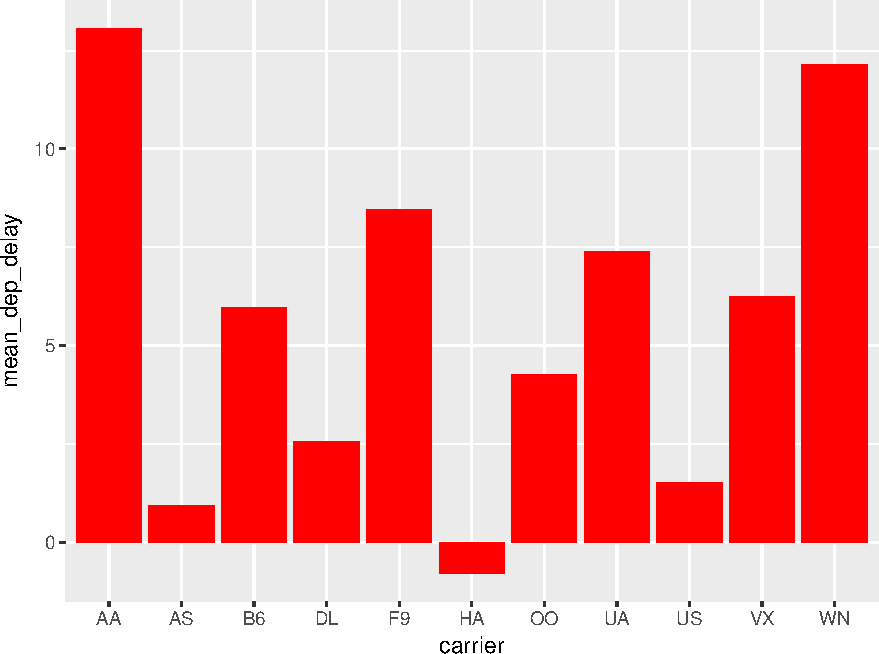
\includegraphics{thesis_files/figure-latex/delaysboxplot-1.pdf}
\caption{\label{fig:delaysboxplot}Mean Delays by Airline}
\end{figure}
Here is a reference to this image: Figure \ref{fig:delaysboxplot}.

A table linking these carrier codes to airline names is available at
\url{https://github.com/ismayc/pnwflights14/blob/master/data/airlines.csv}.

\clearpage

Next, we will explore the use of the \texttt{out.extra} chunk option,
which can be used to shrink or expand an image loaded from a file by
specifying \texttt{"scale=\ "}. Here we use the mathematical graph
stored in the ``subdivision.pdf'' file.
\begin{figure}
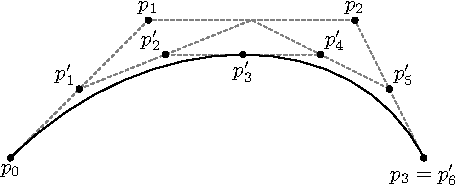
\includegraphics[scale=0.75]{figure/subdivision} \caption{Subdiv. graph}\label{fig:subd}
\end{figure}
Here is a reference to this image: Figure \ref{fig:subd}. Note that
\texttt{echo=FALSE} is specified so that the \textbf{R} code is hidden
in the document.

\textbf{More Figure Stuff}

Lastly, we will explore how to rotate and enlarge figures using the
\texttt{out.extra} chunk option. (Currently this only works in the PDF
version of the book.)
\begin{figure}
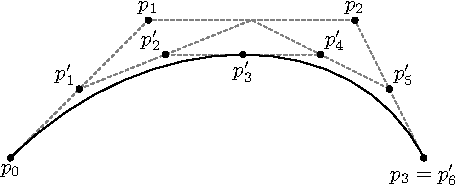
\includegraphics[angle=180, scale=1.1]{figure/subdivision} \caption{A Larger Figure, Flipped Upside Down}\label{fig:subd2}
\end{figure}
As another example, here is a reference: Figure \ref{fig:subd2}.

\section{Footnotes and Endnotes}\label{footnotes-and-endnotes}

You might want to footnote something.\footnote{footnote text} The
footnote will be in a smaller font and placed appropriately. Endnotes
work in much the same way. More information can be found about both on
the CUS site or feel free to reach out to
\href{mailto:data@reed.edu}{\nolinkurl{data@reed.edu}}.

\section{Bibliographies}\label{bibliographies}

Of course you will need to cite things, and you will probably accumulate
an armful of sources. There are a variety of tools available for
creating a bibliography database (stored with the .bib extension). In
addition to BibTeX suggested below, you may want to consider using the
free and easy-to-use tool called Zotero. The Reed librarians have
created Zotero documentation at
\url{http://libguides.reed.edu/citation/zotero}. In addition, a tutorial
is available from Middlebury College at
\url{http://sites.middlebury.edu/zoteromiddlebury/}.

\emph{R Markdown} uses \emph{pandoc} (\url{http://pandoc.org/}) to build
its bibliographies. One nice caveat of this is that you won't have to do
a second compile to load in references as standard LaTeX requires. To
cite references in your thesis (after creating your bibliography
database), place the reference name inside square brackets and precede
it by the ``at'' symbol. For example, here's a reference to a book about
worrying: (Molina \& Borkovec, 1994). This \texttt{Molina1994} entry
appears in a file called \texttt{thesis.bib} in the \texttt{bib} folder.
This bibliography database file was created by a program called BibTeX.
You can call this file something else if you like (look at the YAML
header in the main .Rmd file) and, by default, is to placed in the
\texttt{bib} folder.

For more information about BibTeX and bibliographies, see our CUS site
(\url{http://web.reed.edu/cis/help/latex/index.html})\footnote{Reed~College
  (2007)}. There are three pages on this topic: \emph{bibtex} (which
talks about using BibTeX, at
\url{http://web.reed.edu/cis/help/latex/bibtex.html}),
\emph{bibtexstyles} (about how to find and use the bibliography style
that best suits your needs, at
\url{http://web.reed.edu/cis/help/latex/bibtexstyles.html}) and
\emph{bibman} (which covers how to make and maintain a bibliography by
hand, without BibTeX, at
\url{http://web.reed.edu/cis/help/latex/bibman.html}). The last page
will not be useful unless you have only a few sources.

If you look at the YAML header at the top of the main .Rmd file you can
see that we can specify the style of the bibliography by referencing the
appropriate csl file. You can download a variety of different style
files at \url{https://www.zotero.org/styles}. Make sure to download the
file into the csl folder.

\textbf{Tips for Bibliographies}
\begin{itemize}
\tightlist
\item
  Like with thesis formatting, the sooner you start compiling your
  bibliography for something as large as thesis, the better. Typing in
  source after source is mind-numbing enough; do you really want to do
  it for hours on end in late April? Think of it as procrastination.
\item
  The cite key (a citation's label) needs to be unique from the other
  entries.
\item
  When you have more than one author or editor, you need to separate
  each author's name by the word ``and'' e.g.
  \texttt{Author\ =\ \{Noble,\ Sam\ and\ Youngberg,\ Jessica\},}.
\item
  Bibliographies made using BibTeX (whether manually or using a manager)
  accept LaTeX markup, so you can italicize and add symbols as
  necessary.
\item
  To force capitalization in an article title or where all lowercase is
  generally used, bracket the capital letter in curly braces.
\item
  You can add a Reed Thesis citation\footnote{Noble (2002)} option. The
  best way to do this is to use the phdthesis type of citation, and use
  the optional ``type'' field to enter ``Reed thesis'' or
  ``Undergraduate thesis.''
\end{itemize}
\section{Anything else?}\label{anything-else}

If you'd like to see examples of other things in this template, please
contact the Data @ Reed team (email
\href{mailto:data@reed.edu}{\nolinkurl{data@reed.edu}}) with your
suggestions. We love to see people using \emph{R Markdown} for their
theses, and are happy to help.

\chapter*{Conclusion}\label{conclusion}
\addcontentsline{toc}{chapter}{Conclusion}

If we don't want Conclusion to have a chapter number next to it, we can
add the \texttt{\{-\}} attribute.

\textbf{More info}

And here's some other random info: the first paragraph after a chapter
title or section head \emph{shouldn't be} indented, because indents are
to tell the reader that you're starting a new paragraph. Since that's
obvious after a chapter or section title, proper typesetting doesn't add
an indent there.

\appendix

\chapter{The First Appendix}\label{the-first-appendix}

This first appendix includes all of the R chunks of code that were
hidden throughout the document (using the \texttt{include\ =\ FALSE}
chunk tag) to help with readibility and/or setup.

\textbf{In the main Rmd file}

\textbf{In Chapter \ref{ref-labels}:}
\begin{Shaded}
\begin{Highlighting}[]
\CommentTok{# This chunk ensures that the thesisdown package is}
\CommentTok{# installed and loaded. This thesisdown package includes}
\CommentTok{# the template files for the thesis and also two functions}
\CommentTok{# used for labeling and referencing}
\NormalTok{if(!}\KeywordTok{require}\NormalTok{(devtools))}
  \KeywordTok{install.packages}\NormalTok{(}\StringTok{"devtools"}\NormalTok{, }\DataTypeTok{repos =} \StringTok{"http://cran.rstudio.com"}\NormalTok{)}
\NormalTok{if(!}\KeywordTok{require}\NormalTok{(dplyr))}
    \KeywordTok{install.packages}\NormalTok{(}\StringTok{"dplyr"}\NormalTok{, }\DataTypeTok{repos =} \StringTok{"http://cran.rstudio.com"}\NormalTok{)}
\NormalTok{if(!}\KeywordTok{require}\NormalTok{(ggplot2))}
    \KeywordTok{install.packages}\NormalTok{(}\StringTok{"ggplot2"}\NormalTok{, }\DataTypeTok{repos =} \StringTok{"http://cran.rstudio.com"}\NormalTok{)}
\NormalTok{if(!}\KeywordTok{require}\NormalTok{(ggplot2))}
    \KeywordTok{install.packages}\NormalTok{(}\StringTok{"bookdown"}\NormalTok{, }\DataTypeTok{repos =} \StringTok{"http://cran.rstudio.com"}\NormalTok{)}
\NormalTok{if(!}\KeywordTok{require}\NormalTok{(thesisdown))\{}
  \KeywordTok{library}\NormalTok{(devtools)}
  \NormalTok{devtools::}\KeywordTok{install_github}\NormalTok{(}\StringTok{"ismayc/thesisdown"}\NormalTok{)}
  \NormalTok{\}}
\KeywordTok{library}\NormalTok{(thesisdown)}
\NormalTok{flights <-}\StringTok{ }\KeywordTok{read.csv}\NormalTok{(}\StringTok{"data/flights.csv"}\NormalTok{)}
\end{Highlighting}
\end{Shaded}
\chapter{The Second Appendix, for
Fun}\label{the-second-appendix-for-fun}

\backmatter

\chapter*{References}\label{references}
\addcontentsline{toc}{chapter}{References}

\markboth{References}{References}

\noindent

\setlength{\parindent}{-0.20in} \setlength{\leftskip}{0.20in}
\setlength{\parskip}{8pt}

\hypertarget{refs}{}
\hypertarget{ref-angel2000}{}
Angel, E. (2000). \emph{Interactive computer graphics : A top-down
approach with opengl}. Boston, MA: Addison Wesley Longman.

\hypertarget{ref-angel2001}{}
Angel, E. (2001a). \emph{Batch-file computer graphics : A bottom-up
approach with quicktime}. Boston, MA: Wesley Addison Longman.

\hypertarget{ref-angel2002a}{}
Angel, E. (2001b). \emph{Test second book by angel}. Boston, MA: Wesley
Addison Longman.

\hypertarget{ref-Molina1994}{}
Molina, S. T., \& Borkovec, T. D. (1994). The Penn State worry
questionnaire: Psychometric properties and associated characteristics.
In G. C. L. Davey \& F. Tallis (Eds.), \emph{Worrying: Perspectives on
theory, assessment and treatment} (pp. 265--283). New York: Wiley.

\hypertarget{ref-noble2002}{}
Noble, S. G. (2002). \emph{Turning images into simple line-art}
(Undergraduate thesis). Reed College.

\hypertarget{ref-reedweb2007}{}
Reed~College. (2007, march). LaTeX your document. Retrieved from
\url{http://web.reed.edu/cis/help/LaTeX/index.html}


% Index?

\end{document}
